\documentclass[tikz,border=8pt]{standalone}
\usepackage{amsmath,amssymb}
\usetikzlibrary{arrows.meta,calc,patterns}

\begin{document}
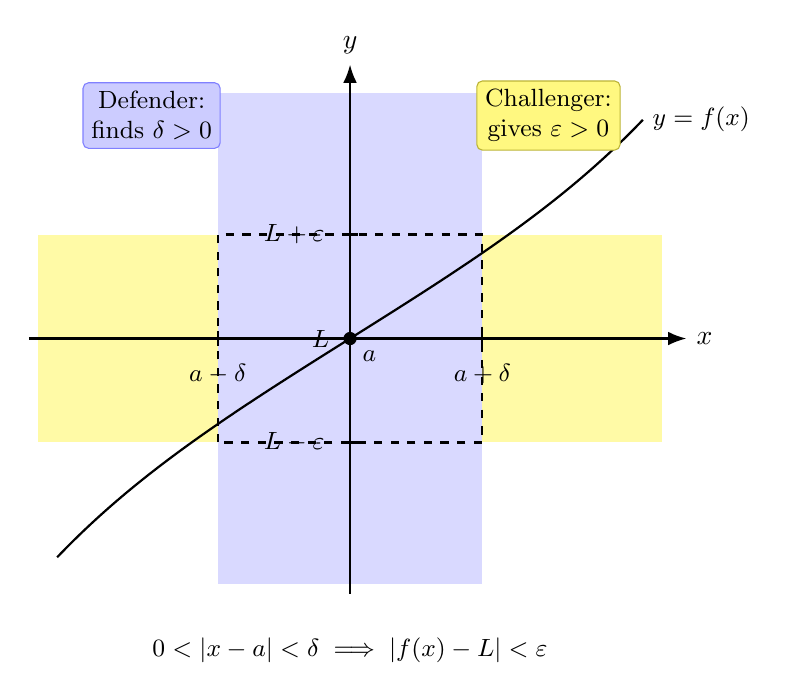
\begin{tikzpicture}[scale=2.4,>=Latex]
  \def\eps{0.55}
  \def\del{0.7}

  % epsilon-band (horizontal yellow)
  \fill[yellow!35] (-1.65,-\eps) rectangle (1.65,\eps);
  % delta-band (vertical blue)
  \fill[blue!15] (-\del,-1.3) rectangle (\del,1.3);
  % intersection rectangle (dashed)
  \draw[dashed, thick] (-\del,-\eps) rectangle (\del,\eps);

  % axes
  \draw[->,thick] (-1.7,0)--(1.78,0) node[right]{$x$};
  \draw[->,thick] (0,-1.35)--(0,1.45) node[above]{$y$};

  % function curve: smooth, passes through (0,0), exits eps-band beyond delta
  \draw[thick, black, smooth, samples=120, domain=-1.55:1.55]
        plot(\x, {0.6*sin(60*\x) + 0.15*\x*\x*\x});

  % point (a, L)
  \fill[black] (0,0) circle (0.035);

  % tick marks
  \draw[thick] (-\del,0.04)--(-\del,-0.04);
  \draw[thick] (\del,0.04)--(\del,-0.04);
  \draw[thick] (0.04,\eps)--(-0.04,\eps);
  \draw[thick] (0.04,-\eps)--(-0.04,-\eps);

  % labels on axes
  \node[below=3pt, font=\small] at (-\del,-0.04) {$a-\delta$};
  \node[below=3pt, font=\small] at (\del,-0.04) {$a+\delta$};
  \node[below right=1pt, font=\small] at (0,0) {$a$};
  \node[left=3pt, font=\small] at (-0.04,\eps) {$L+\varepsilon$};
  \node[left=3pt, font=\small] at (-0.04,-\eps) {$L-\varepsilon$};
  \node[left=4pt, font=\small] at (0,0) {$L$};

  % game annotations
  \node[align=center, font=\small, fill=yellow!50, rounded corners=2pt, inner sep=3pt, draw=yellow!70!black] at (1.05,1.18)
    {Challenger:\\gives $\varepsilon>0$};
  \node[align=center, font=\small, fill=blue!20, rounded corners=2pt, inner sep=3pt, draw=blue!50] at (-1.05,1.18)
    {Defender:\\finds $\delta>0$};

  % formula at bottom
  \node[font=\small] at (0,-1.65)
    {$0<|x-a|<\delta \;\Longrightarrow\; |f(x)-L|<\varepsilon$};

  % function label
  \node[font=\small,right] at (1.55,1.16) {$y=f(x)$};
\end{tikzpicture}
\end{document}
